\chapter{Method}

The work with this thesis can be divided into two parts, the first being reading litterature regarding the Semantic Web, Linked Data and related subjects. The litterature also included reading many articels, blog post and watching podcasts,\footnote{TODO, links to references, podcasts etc.} that were great to get a better understaning of the concept and importance of a more semantic web.\\\\  
The second part was to create a prototyp. Before I started to work on that I looked at the existing system, and tried to get some understanding of what steps the process went through. At this point a I got a lot of guidence from Magnus at Notisum, the author of the existing code. He explained the necessary steps and why they are important for the end result. However I didn't spend to much time on the old code, since I needed to create something different (and take factors such as semantics into mind).\\ With no background or knowledge in law it can be quite hard to understand the structure of laws and references between them. That is something I picked up as work went along with the prototype, many times I had to stop and try to figure out what I tried to do and why. 

\section{Methodology}
I devloped the prototype in several iterations, a simplfied version of agile.\footnote{Agile ... TODO} The first step was to get the program to read downloaded documents and save them as a new file. After that was in place, I always had a running prototype that would go through all files in a specified folder and apply transformations to them before saving them with a new exstension. This way I could add new functionality and try it out right away. I tried to put general functions and helpers seperate from SFS-specific logic so that it is possible to reuse a lot of the code when other legal sources needs to be implemented.     

\section{Existing system}
Below follows a short description of the steps the process goes through today. The steps in blue bubbles (first and last) are written in C\# and could with minor modifications be used together with the prototype. The two steps in pink bubbles (second step which is split in two different parts and the third step) are programs written in Pascal and will be replaced by the prototype. Then there's a green bubble (fourth step) which also with some modifications, could be reused with the output from the prototype.   
\begin{center}
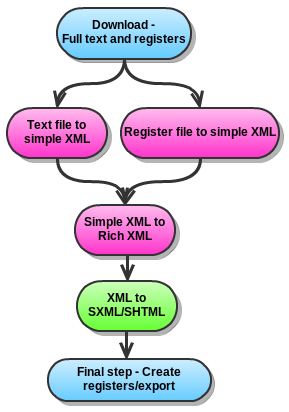
\includegraphics[scale=0.6]{../imgs/oldSystemChart.png}
\captionof{figure}{Chart describing the existing process}
\end{center}
For the sake of simplicity lets say we are only handling SFS laws\footnote{In reality the program handles all kind of legal source documents.}. First we have a module that handles the actual downloading of the legal source files, (full text and register files\footnote{TODO, explain Registerfile} for each law) this part is written in C\# and could be reused\footnote{This part just have to download the files, then the prototype can do it's magic on those files.} for the prototype. Next we have two programs that for each law converts the downloaded files to very simple XML files, one for the full text and one for the registerfile. The next step is also an XML transformation, it takes the simple XML files and turns them into more comprehensive XML files. Now it's time to create files that can be viewed in a browser, this is done in several steps where data structures containing information regarding the laws are created with information like paragraph references and links. In the end a SHTML\footnote{TODO, explain SHTML} file that is ready to be published with this information is created. The final step is to export these files (and other legal source documents) to databases and update the website to display the newly created or updated files.

\section{Prototype}
The main differences between the old system and the prototype are: 
\begin{itemize}
\item Language, the prototype is written in Python\footnote{TODO, something about python} which is a object oriented\footnote{something about OO} languge that is well suited for tasks like this one. It is easy to divide the code into separate modules that handle different tasks. Furthermore it is convinient to work with (apply transformations etc.) objects such as whole documents, paragraphs. 
\item Follows standards proposed by Rättsinformationsprojektet for legal documents.   
\item RDF, TODO: Marked up with URI's to.. 
\end{itemize} 

\subsection{Delimitations}
The prototype does not have to handle the downloading of the legal source documents, these can be presumed exist on the computer running the prototype. \\The aim for the prototype is to deliver XML files, the final step where these files are transformed into HTML files is simple and needs to be controlled by Notisum. However this step is done by the prototype but might not be the way Notisum will do it, if they use the prototype.